%%%%%%%%%%%%%%%%%%%%% chapter.tex %%%%%%%%%%%%%%%%%%%%%%%%%%%%%%%%%
%
% sample chapter
%
% Use this file as a template for your own input.
%
%%%%%%%%%%%%%%%%%%%%%%%% Springer-Verlag %%%%%%%%%%%%%%%%%%%%%%%%%%
%\motto{Use the template \emph{chapter.tex} to style the various elements of your chapter content.}
\chapter{Cut \& Count für das Steinerbaum-Problem}
\label{c:cc_steiner}

\section{Steinerbaum}
\label{sec:steiner}
\begin{definition}
Steinerbaum-Problem\\
\textbf{Eingabe}: Sei $G = (V, E)$ ein ungerichteter Graph, $T \subseteq V$ eine Menge von Terminalknoten und $k$ eine positive Ganzzahl. \\
\textbf{Problemstellung}: Gibt es eine Menge $X \subseteq V$ der Kardinalität $k$, so dass $T \subseteq X$ und $G[X]$ zusammenhängend ist?
\end{definition}

In einem gegebenen Graphen ist eine Menge $T \subseteq V$ als Terminale markiert. Gesucht ist ein Subgraph innerhalb des Ursprungsgraphen, der alle Terminale enthält und genau $k$ Knoten enthält. Zudem muss der Subgraph zusammenhängend sein, es muss also jeder Knoten von jedem anderen Knoten des Subgraphen über einen Pfad innerhalb des Subgraphen erreichbar sein.

\section{Cut}
\label{sec:st_cut}
Zu Beginn des Cut-Teils wird eine zufällige Gewichtsfunktion $\omega:V\rightarrow \{1,\dots,N\}$ definiert. 
Diese wird für die Isolation der Lösungsmenge verwendet. 
$\omega$ weist jedem Knoten zufäälig ein Gewicht zu. 
Wird $\omega$ auf eine Menge von Knoten angewendet, ist das Ergebnis die Summe der einzelnen Knotengewichte.\\
Anschließend definieren wir die Menge $\mathcal{R}$, welche die Zusammenhangs-Bedingung abschwächt. 
Somit ist $\mathcal{R}_W$ die Menge aller Teilmengen von $X$ aus $V$ mit $T \subseteq X$, $\omega(X)=W$ und $|X|=k$. Die Menge $\mathcal{R}_W$ beschreibt alle Lösungskandidaten.\\
Die Menge $\mathcal{S}_W=\{X \in \mathcal{R}_W | G[X]$ ist zusammenhängend$\}$ umfasst die Lösungsmenge für eine Menge $\mathcal{R}_W$. 
$\cup_W \mathcal{S}_W$ bildet so die gesamte Lösungsmenge. 
Gibt es ein Gewicht $W$ für das die Menge nicht leer ist, so gibt der Algorithmus eine positive Antwort.\\
Von der Menge der Terminalknoten wird ein zufälliges Terminal als $v_1$-Terminal festgelegt. 
Dieses dient dazu, dass bei der Bildung von konsistenten Schnitten kein Schnitt doppelt gezählt wird.\\
Ein Schnitt $(V_1,V_2)$ eines ungerichteten Graphen $G=(V,E)$ ist konsistent, falls $u \in V_1$ und $v \in V_2$ impliziert, dass $uv \notin E$. 
Ein Subgraph, der einen konsistenten Schnitt aus $G$ bildet, ist ein Paar $(X,(X_1,X_2))$, so dass $(X_1,X_2)$ ein konsistenter Schnitt von $G[X]$ ist.
$\mathcal{C}_W$ sei die Menge aller Subgraphen, die einen konsistenten Schnitt $(X,(X_1,X_2))$ bilden, wobei $X\in \mathcal{R}_W$ und $v_1 \in X_1$.
\begin{figure}
  \centering
    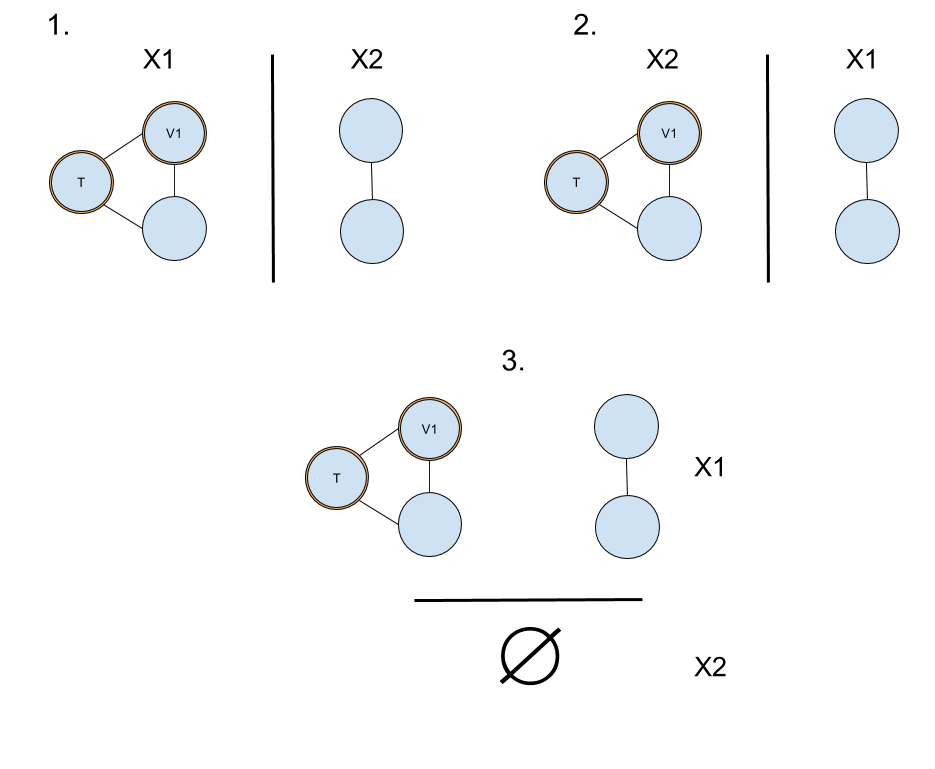
\includegraphics[width=0.5\textwidth]{./imgs/terminal_v1.png}
  	\caption{Konsistente Schnitte}
	\label{fig:st_cut}
\end{figure}

Die Anzahl der Subgraphen, welche einen konsistenten Schnitte bilden, sind in Lemma 3.3 in \cite{cygan_solving_2011} definiert:

Let $G=(V,E)$ be a graph and let $X$ be a subset of vertices such that $v_1 \in X \subseteq V$. The number of consistently cut subgraphs $(X,(X_1,X_2))$ such that $v_1 \in X_1$ is equal to $2^{cc(G[X])-1}$.

Ausgehend von der Definition $\mathcal{C}_W$ ist für jeden Subgraphen, der einen konsistenten Schnitt $(X,(X_1,X_2))$ bildet, und für jede Zusammenhangskomponente $C$ aus $G[X]$ bekannt, dass  $C$ entweder in $X_1$ oder in $X_2$ enthalten sein muss. Für die Zusammenhangskomponente, die $v_1$ enthält, ist die Seite des Schnitts fest. Für alle anderen Zusammenhangskomponenten kann die Seiten der Mengen $X_1,X_2$ frei gewählt werden. Daher erhalten wir $2^{cc(G[X])-1}$ verschiedene konsistente Schnitte.

In der Abbildung \ref{fig:st_cut} zeigt beispielhaft die Bildung von konsistenten Schnitten. Die getrichelte und gepunktete Line veranschaulicht den konsistenten Schnitt visuell. Die Knoten mit doppeltem Rand stellen Terminale da. Das Terminal $A$ wird als $v_1$ Terminal festgelegt. Zur Vereinfachung wurde die Gewichte der Knoten ignoriert.
Aus diesem Beispiel gehen mit $k=3$ folgende Mengen hervor:
\begin{itemize}
\item $\mathcal{R} = \{\{A,B,C\}, \{A,B,D\}, \{A,B,E\}\}$
\item $\mathcal{S} = \{\{A,B,C\}\}$
\end{itemize}

Aus der $\mathcal{R}$ Menge ergeben sich folgende $\mathcal{C}$ Mengen:
\begin{itemize}
\item Für $\mathcal{R}_1$:
\begin{itemize}
\item $\mathcal{C}_{1.1} = \{(A,B,C),  (\{A,B,C\}, \{\emptyset\})\}$
\end{itemize}
\item Für $\mathcal{R}_2$:
\begin{itemize}
\item $\mathcal{C}_{2.1} = \{(A,B,D),  (\{A,B\}, \{D\})\}$
\item $\mathcal{C}_{2.2} = \{(A,B,D),  (\{A,B,D\}, \{\emptyset\})\}$ 
\end{itemize}
\item Für $\mathcal{R}_3$:
\begin{itemize}
\item $\mathcal{C}_{3.1} = \{(A,B,E),  (\{A,B\}, \{E\})\}$
\item $\mathcal{C}_{2.1} = \{(A,B,D),  (\{A,B,E\}, \{\emptyset\})\}$
\end{itemize}
\end{itemize}

Ohne die Restriktion $v_1 \in X_1$ gäbe es die doppelte Menge an konsistenten Schnitten. Bei jedem Schnitt könnte die Mengen $X_1$ und $X_2$ vertauscht werden. Durch die Restriktion von $v_1$ wird dies vermieden.


\section{Count}
\label{sec:st_count}
Aus Lemma 3.3 ist bekannt: $|\mathcal{C}|=\sum_{X \in \mathcal{R}} 2^{cc(G[X])-1}$. \\
Durch die Randomisierung mithilfe der Knotengewichte wird die Wahrscheinlichkeit, dass die Menge der Lösungskandidaten $\mathcal{R}$ mehrere Lösungen enthält, reduziert. 
Für eine Lösung $\mathcal{S} \in \mathcal{R}$ gilt, dass $G[X]$ zusammenhängend ist. 
Durch die Festlegung des $v_1$-Terminals wird zudem die Möglichkeit des Schnitts für eine Lösung auf eins reduziert (Schnitt mit der leeren Menge). 
Daher gilt $|\mathcal{S}| = |\{X \in \mathcal{R}\}| cc(G[X]=1)$.
Also können wir schreiben: $|\mathcal{C}_W| \equiv |\mathcal{S}_W|$.

Diese Äquivalenz erlaubt es ein dynamisches Programm zu beschreiben, dass nicht die Menge der Lösungen $\mathcal{S}$, sondern die Anzahl der Subgraphen $|\mathcal{C}_W|$, die einen konsistenten Schnitt bilden, zu berechnen. Dieses Programm ist in folgender Sektion näher erläutert.
%Wir legen $W$ fest und ignorieren die Indices: $|\mathcal{C}| \equiv |\{X \in \mathcal{R} |cc(G[X]) = 1\}| = |\mathcal{S}|$. 
%Das bedeutet, dass die Anzahl der konsistenten Schnitte eines Graphen modulo zwei gleich der Anzahl der Lösungen ist. 
%Im Lemma 3.4 trifft das Paper dazu eine Aussage: Let $G,$ $\omega$, $\mathcal{C}_W$ and $\mathcal{S}_W$ be as defined above. 
%Then for every $W$, $|\mathcal{S}_W| \equiv |\mathcal{C}_W|$.

\section{Dynamisches Programm}
\label{sec:dynP}

Für das dynamische Programm werden für jeden Bag $x \in \mathbb{T}$, die Zahlen $0 \leq i \leq k,0 \leq w \leq kN$ und die Färbung $s \in \{0,1_1,1_2 \}^{B_x}$ folgende Mengen definiert:
\begin{itemize}
\item $\mathcal{R}_x(i,w)=\{X \subseteq V_x | (T \cap V_x) \subseteq X$ $\wedge$ $|X| = i$ $\wedge$ $\omega (X) = w \}$ \\
beschreibt die Menge der Lösungskandidaten
\item $\mathcal{C}_x (i,w) =\{ (X,(X_1,X_2)) | X \in \mathcal{R}_x(i,w)$ $\wedge$ $(X,(X_1,X_2))$ ist ein Subgraph, der einen konsistenten Schnitt von $G_x$ bildet $\wedge$ $(v_1 \in V_x \Rightarrow v_1 \in X_1 \} $
\item $\mathcal{A}_x(i,w,s)=| \{ (X,(X_1,X_2)) \in \mathcal{C}_x(i,w) | (s(v) = 1_j \Rightarrow v \in X_j)$ $\wedge$ $(s(v)=0 \Rightarrow v \notin X \} |$ \\
beschreibt die Anzahl der Mengen $\mathcal{C}_x(i,w)$, wobei die in $X$ enthaltenen Knoten mit $s \in \{1_1,1_2\}$ gefärbt sind und die restlichen Knoten mit $s=0$ 
\end{itemize}
Die Färbung gibt an, ob und zu welcher Seite eines konsistenten Schnitts ein Knoten gehört.
Die Zuordnung der Färbung $s \in \{0,1_1,1_2 \}^{B_x}$  der Knoten aus Bag $B_x$ bzgl. der Menge $C_x$ ist folgendermaßen definiert:
\begin{itemize}
\item $s[v] = 0 \Rightarrow v \notin X$
\item $s[v] = 1_1 \Rightarrow v \in X_1$ 
\item $s[v] = 1_2 \Rightarrow v \in X_2$ 
\end{itemize}
$A_x(i,w,s)$ zählt alle Möglichkeiten die Knoten eines Bags $x$ gemäß der Definition zu färben. Es gibt für einen Bag $3^{B_x}$ Möglichkeiten die Knoten zu färben.

Im dynamischen Programm werden die folgenden Berechnungsregeln für jede $A_x(i,w,s)$ Matrix eines Bags $x$ angewandt. Zur Vereinfachung der Notation beschreibt im folgenden $v$ den neu eingeführten Vertex. $y$ und $z$ stehen für das linke bzw. das rechte Kind:
\begin{itemize}
\item \textbf{Leaf bag}:
\begin{itemize}
\item $A_x=(0,0,\emptyset) = 1$\\Leaf bags enhalten keine Knoten, daher werden sie mit einem Initialwert gefüllt.
\end{itemize}
\item \textbf{Introduce vertex v}:
\begin{itemize}
\item $A_x=(i,w,s[v\rightarrow 0]) = [v \notin T]A_y(i,w,s)$\\ Ist der eingeführte Vertex kein Terminal, so wird der Wert aus dem Bag des Kindes übernommen.
\item $A_x=(i,w,s[v\rightarrow 1_1]) = A_y(i-1,w-w(v),s)$\\ Reduziere beim Zugriff auf den Bag des Kindes i um 1 und ziehen das Gewicht des eingeführten Knoten ab. Übernehme den Wert.
\item $A_x=(i,w,s[v\rightarrow 1_2]) =[v \neq v_1] A_y(i-1,w-w(v),s)$\\ Ist der eingeführte Vertex nicht das speziell gewählte Terminal so verfahre wie bei $1_1$.
\end{itemize}
\item \textbf{Introduce edge uv}
\begin{itemize}
\item $A_x(i,w,s) = [s(u) = 0 \vee s(v) = 0 \vee s(u) = s(v)]A_y(i,w,s)$\\ Ist einer der Verticies $0$ gefärbt oder sind beide gleich gefärbt, so wird der Wert aus dem Bag des Kindes übernommen.
\end{itemize}
\item \textbf{Forget vertex v}
\begin{itemize}
\item $A_x(i,w,s) = \sum\limits_{\alpha \in {0,1_1,1_2}} A_x(i,w,s[v \rightarrow \alpha]) $\\ Es wird die Summe gebildet über alle Färbungen des vergessenen Vertex im Bag des Kindes.
\end{itemize}
\item \textbf{Join bag}
\begin{itemize}
\item $A_x(i,w,s) = \sum\limits_{i_1+i_2=i+|s^{-1}({1_1,1_2})|}$   $\sum\limits_{w_1+w_2=w+w(s^{-1}({1_1,1_2}))} A_y(i_1,w_1,s)A_z(i_2,w_2,s) $\\In der inneren Summe wird über die Gewichte innerhalb beider Bags der Kinder iteriert. Ist deren Summe gleich der Summe von $w$ und der Summe der Gewichte von Knoten mit der Färbung $1_1$ und $1_2$, so werden sie akkumuliert.
\\In der äußeren Summe wird über den Parameter $i$ der Bags der Kinder iteriert. Ist die Summe gleich der Summe von $i$ und der Anzahl der Knoten die $1_1$ und $1_2$ gefärbt sind, so werden sie akkumuliert.
\end{itemize}
\end{itemize}


Ob der Algorithmus eine Lösung gefunden hat, kann aus der $k \times kN$-Datenmatrix des Wurzel-Knotens $A_r(i,w,\emptyset)$ ausgelesen werden. 
Dieser Zugriff ist konstant in $\mathcal{O}(1)$.\\
Falls eine Lösung existiert und diese gefunden wurde, dann existiert ein $0 \leq W \leq kN$ für das $A_r(k,W,\emptyset) \equiv 2 = 1$.

\section{Monte-Carlo Algorithmus und Laufzeit}
\label{sec:mc_alg}
Im Theorem 3.6 des Papers wird zusammenfassend erwähnt:
\begin{theorem}
There exists a Monte-Carlo algorithm that given a tree decomposition of width $t$ solves STEINER TREE in $3^t|V|^{\mathcal{O}(1)}$ time. The algorithm cannot give false positives and may give false negatives with probability at most 1/2.
\end{theorem}

Die Laufzeit setzt sich wie folgt zusammen, wobei $t$ für die Baumweite der NTD steht.
\begin{itemize}
\item $3^t$:\\ Für jeden Bag muss über alle Farbkombinationen iteriert werden. Die obere Grenze hierbei ist die Anzahl der Knoten im größten Bag. Dieser besitzt $3^t$ verschiedene Färbungen.
\item $|V|^{\mathcal{O}(1)}$:\\ obere Grenze der Eingabe-Parameter k und N.
\item Die Wahrscheinlichkeit von 1/2 für falsch-negativ entsteht durch die Gewichtsfunktion $\omega:V\rightarrow \{1,\dots,N\}$ und durch das Isolations-Lemma, sofern $N=2|V|$ gesetzt wird. 
\end{itemize}